\section{Introduction}

\flushleft \justifying Chronic Kidney Disease (CKD) is very prevalent today. Almost 15\% of Americans i.e. Thirty-seven million Americans currently have Chronic Kidney Disease (CKD). An increasing number of people are at an increased risk of having CKD. People who have diabetes, Hypertension as well as smokers, and those over 60 are at an increased risk of developing CKD. CKD can lead to End Stage Renal Disease (ESRD), kidney failure, and death. CKD/ESRD and interrelated diseases such as Hypertension, Heart Disease, and Diabetes lead to a majority of early deaths. In addition, CKD is also a primary cause of death from stroke and heart disease. CKD has no permanent cure. CKD is not reversible. It is progressive and leads to kidney failure eventually. Hence, CKD treatment involves drugs, lifestyle, and food choices and slows the progression. Because food can also affect CKD progression, studying the effect of food choices on CKD is important. Hence, this study focused on studying the effect of Food groups on CKD. We selected a CKD diagnostic marker such as Urine Albumin Creatinine Ratio and studied the effect of Food Groups on ACR.

\flushleft \justifying The majority of the research studied the effects of Drugs and nutrients on CKD progression. The effect of food and eating patterns on CKD has attracted recent attraction. However, the research is not significant yet. Additional research is required to understand how Food and Lifestyle choices affect CKD. Hence, in this study, we have studied the effect of food groups on a CKD diagnostic marker called Urine Albumin Creatinine Ratio (ACR). In addition, we have clustered and grouped the data based on Demographics characteristics such as age as well as CKD stages based on ACR readings. We noticed that Medical studies use age groups in steps of 10 years, 4 years, or 30 years. We have adopted the 30 years steps. Several CKD studies clustered the population based on various CKD patient characteristics. However, this research identified the vulnerable clusters in terms of risks of facing severity. I did not come across any study utilizing the same dataset as ours and using clustering to find relations of food groups with ACR. However, we also have considered utilizing clustering approaches such as K-means to identify 10 groups where age and ACR readings can be the centers to create the clusters. Using these clusters, we can find out the relations of ACR with Food Groups. In addition, we can identify the vulnerable groups most sensitive to ACR readings for food groups. Our K-Means clustering algorithm is provided in the methodology section.

\flushleft \justifying CKD is measured using diagnostic markers such as Glomerular Filtration Rate (GFR) and Urine Albumin Creatinine ratio. GFR readings range between 1 and 120. GFR divided CKD into five stages such as Stage 1 ( GFR = 90 to 120 mL/min), Stage 2 ( GFR = 60 to 90 mL/min), Stage 3 (GFR = 30 to 60 mL/min), Stage 4 ( GFR = 15 to 30 mL/min), and Stage 5 ( GFR = 0 to 15 mL/min). Stage 5 is the most severe. At this stage, patients lose kidney function and require either dialysis or organ transplantation for survival. ACR also determines the severity of CKD in stages such as Stage 1 (0, $<$ 3), Stage 2 (3, 30), and Stage 3 (30 to 300). Stage 3 is the most severe. ACR values less than 30 i.e. Stage 1 indicates no or mild CKD. ACR values from 30 to 300 i.e Stage 2 indicate moderate CKD. ACR values over 300 i.e Stage 3 indicate severe CKD. Patients are diagnosed with CKD disease if the ACR values persist within the above ranges for three months. CKD severity is also measured in a combination of these two. The severity and how it progresses with both GFR and ACR are shown in Figure ~\ref{gfr-acr-ckd}.

\begin{figure}
\begin{tabular}{cc}
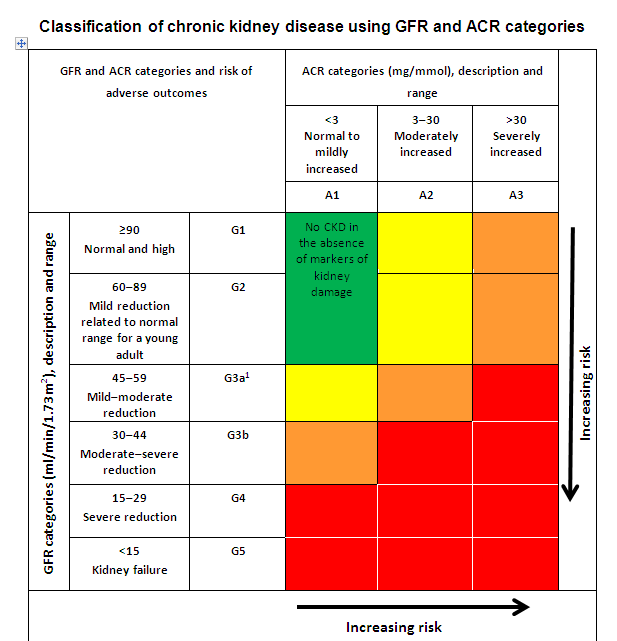
\includegraphics[scale=0.5]{images/gfr-acr-combined-effect.png} & 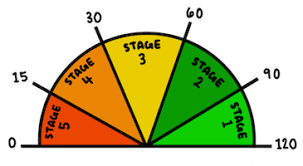
\includegraphics[scale=1.2]{images/gfr1.png} \\
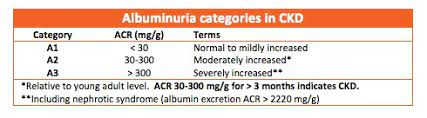
\includegraphics[scale=0.5]{images/acr-stages} & 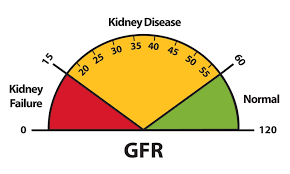
\includegraphics[scale=1.2]{images/gfr2.png} \\
\end{tabular}
\caption{\textbf{GFR, ACR and Kidney Disease (Ref: Google Images)}}
\label{gfr-acr-ckd}
\vspace{0.25cm}
\end{figure}

\flushleft \justifying This study sees how Food Groups affect ACR readings in CKD patients. Moreover, we also wanted to identify what age groups and CKD stages are the most sensitive to food groups. Hence, we studied the effect of Food Groups on ACR for different age groups and CKD stages. Our experiments show no significant relationship between ACR and Food Groups in the population as a whole. We also found that Food Groups show more correlation with ACR for groups with ages under 30 and ACR readings between 3 to 30 than the other groups. In this study, we have utilized Demographics, Dietary Intake, and ACR datasets from NHANES, and CDC. In our study, we have utilized Principle Component Analysis (PCA) to justify the data and find important features in the data. Afterward, we utilized Pearson correlation and regression to study the relation of Food Groups with ACR.

\flushleft \justifying Rest of this report is organized as follows. We will provide a brief literature survey studying the effect of food groups on CKD esp. on ACR and GFR. Additionally, more studies will be mentioned in studies that utilized clustering. Afterward, we will propose our solution and methodology for the study. As part of the solution, we will provide some details about our dataset, data exploration, and dataset generation for our studies. Afterward, we will provide our experimental design. Results and discussion will follow the experimental design. Finally, we will provide discussion and future work.